\chapter{摩托车适配与 T\&B 边界索引：Part 12 改了什么、为什么}

\begin{noteblock}
Semantica 边界： 本附录保存 Part 12 的可读适配说明、两张表的人工转述与教学
走查；书内不再保存或运行 TBox、表实例、SPARQL、SHACL、fixture 或测试脚本。
\nolinkurl{semantica.chapter_packages.vol2.ch04} 只承接本书第 4 章声明的 HARA 场景；当前
\nolinkurl{semantica.chapter_packages.vol2.normative} 只登记已经迁移的 Part 1/Part 3 工程
释义资产，并不声称覆盖 Part 12 全表。因此本附录的 36 格 MSIL 表、5 行映射表及
专项门禁目前没有 released executable successor：任何机器化声称必须先进入新的
Semantica package revision，未完成前保持 unsupported/blocked，绝不调用书内旧路径。
\end{noteblock}

\begin{noteblock}
\textbf{导读}。正文第 4 章的 HARA、S/E/C 与 ASIL 判定都以乘用车为默认舞台。ISO 26262-12:2018（下称 Part 12）回答的问题是：同一套标准搬到摩托车上，哪些条款要换、换成什么、为什么非换不可。读完本附录，你应当能：
1. 说清 Part 12 的适用边界与“替代关系”——它改写了 Parts 2–4 的哪几处，又如何与其余适用要求和工作产物衔接；
2. 独立走一遍摩托车 HARA：用与第 4 章相同的 S/E/C 骨架得出 MSIL，再经映射表落到 ASIL，并解释 MSIL 与 ASIL 为什么不是同义词；
3. 说明卡客车（T\&B）在 Part 12 里的真实地位——只有标记约定，没有适配体系——以及这对想做 T\&B 项目的团队意味着什么。

\textbf{来源性质声明}：与全卷资料性的 Part 11 不同，\textbf{Part 12 的正文条款（Clause 4–10）是规范性的}，含 shall 要求，对适用的摩托车相关项\textbf{取代}其他部的对应要求（§4.5，物理页 p12）；其 Annex A/B/C 为资料性判例与说明（p32、p38、p46）。本附录引用的页码为 1-based 物理页，锚点曾用两种独立生成的提取视图交叉定位；两种视图来自同一份 PDF，不构成两个独立来源。

案例边界：本附录自行构造的判定走查均标注“教学示例”（\nolinkurl{TeachingExample}）；Annex B/C 的示例是资料性判例，不得直接复制为任何项目的 HARA 结论。

\textbf{与全书二十章的衔接}：本书前十章现为叙事重写，方法表语义、独立性等级记号、FMEDA 与失效分类等器具性内容已集中由附录承载；正文各章只提供活动与主题的工程语境。本附录因此按自足深讲编写——凡指向“第 X 章”处均指主题语境，不意味着正文有逐表逐条的展开。
\end{noteblock}


\Needspace{6\baselineskip}
\section{导读：同一套标准为何需要车型适配}

先看一个会把乘用车直觉带进沟里的场景（教学示例）。一份合成的乘用车电子油门 HARA 记录，先把“非预期减速（相当于发动机制动）”在拥堵市区的可控性写成 C1；这个等级只是叙事输入，不代表任何车型或数据库结论。现在同一个功能装上摩托车，团队顺手沿用了那行判定。评审——把工作摊在桌上让同行挑毛病的会议——上被一位骑手出身的工程师拦下：摩托车过弯时车身是\textbf{倾斜}的，轮胎侧向力与纵向力共享附着力预算；弯道中段突然出现的发动机制动会改变纵向载荷与侧向平衡，骑手需要在有限反应窗口内完成判断和姿态修正。这个反问只说明两轮与四轮不能机械复用同一可控性等级；是否改级、改多少，必须由具体场景、车辆与骑手证据支撑。

这就是 Part 12 存在的理由，浓缩成三条摩托车事实：\textbf{动力学不同}——两轮车靠骑手参与才能维持稳定，车辆响应与骑手动作构成一个耦合系统，Part 12 §8.2 明说摩托车的动态行为与标准范围内的其他车辆差异巨大（p20）；\textbf{暴露的人不同}——骑手没有座舱、安全带和气囊，标准假设的防护只有头盔、护具这类穿戴装备（§8.4.3.2 NOTE 5，p22）；\textbf{行业基线不同}——§8.2 的 NOTE 直言：摩托车行业的产品开发过程与技术方案不同于汽车行业，全球已确立的技术水平（state-of-the-art）表明\textbf{直接套 ASIL 分级并不合适}，因此 HARA 的输出改为 MSIL，再经对齐关系映射回 ASIL，以便继续使用其他部的要求（p20）。

注意 Part 12 的克制：它\textbf{没有}重写生命周期。Parts 2–9 构成完整基线，Part 12 在五个技术域提供摩托车专用替代要求：安全文化（Clause 6）、确认措施（Clause 7）、HARA（Clause 8）、整车集成与测试（Clause 9）、安全确认（Clause 10）。这不表示其他要求机械地“原样全做”：仍可按 §4.2 通过安全生命周期裁剪证明某要求不适用，或对可接受的不符合给出并评价理由。本附录按“改了什么、为什么”逐处走查，最后交代 T\&B 的边界。

\Needspace{6\baselineskip}
\section{适配总则与适用边界}

\textbf{替代关系}（§4.5，p12）：对适用 Part 12 要求的摩托车相关项或元素，\textbf{Part 12 的要求取代其他部的对应要求}。这是一条精确的外科手术式规则——取代的只是“对应”的那几条，不是整部标准。§5.2（p12）把对应关系点了名：Part 12 的摩托车专用要求对应 Part 2 的 5.4.2（安全文化）、Part 2 的 6.4.9（确认措施）、Part 3 的 Clause 6 与 Annex B（HARA）、Part 4 的 7.4.4（整车集成测试）与 Part 4 的 Clause 8（安全确认）。除此之外，Parts 2–9 仍是基线，并继续受 §4.2 的裁剪与可接受不符合规则约束——这才是“完整基线 + 五处技术域差分”的准确结构；“五处”不表示 Part 12 的 Clause 4/5 没有规范作用。

\begin{sidewaysfigure}
\centering
\adjustbox{max size={0.92\textheight}{0.85\textwidth}}{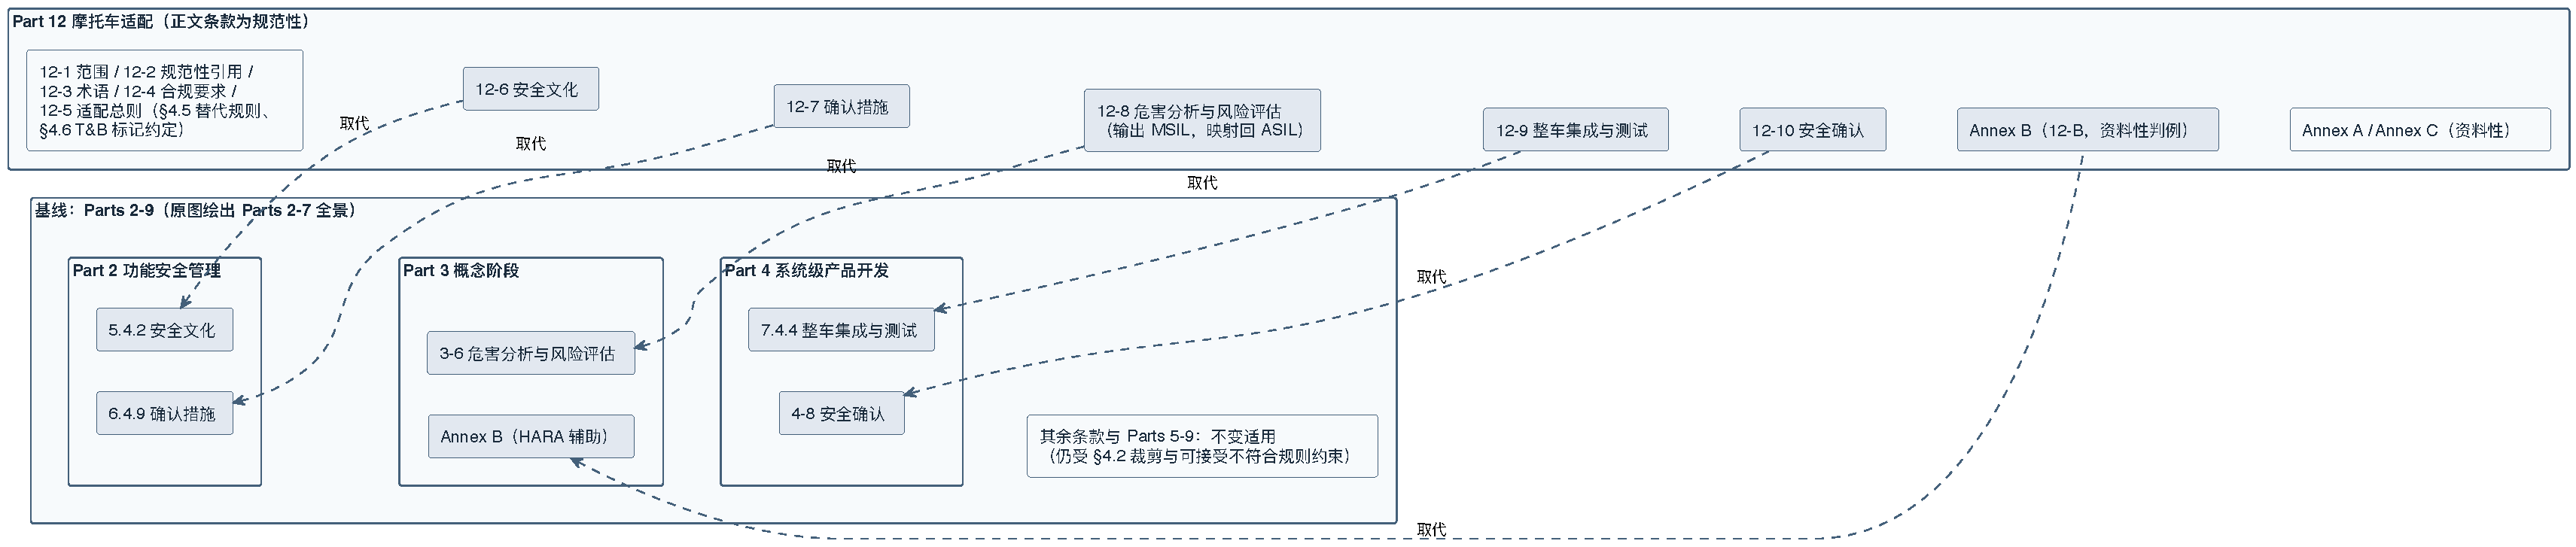
\includegraphics{figures-rendered/appB-fig1-p12-figure2-adaptation-map.pdf}}
\setcounter{figure}{0}
\caption{Part 12 与其他部的替代关系（重绘自 Part 12 Figure 2）——五个技术域条款加 Part 3 Annex B 由 12-6 至 12-10 与 12-B 六条对应逐一取代，其余条款按基线不变适用；重绘压缩了原图的分部全景，对应关系数量与方向保持原图。}
\end{sidewaysfigure}

\textbf{适用范围}（Clause 1，p9）：对象是量产道路车辆上含一个或多个 E/E 系统的安全相关系统，\textbf{不含轻便摩托车（moped）}，也不处理为残障驾驶者等特殊车辆设计的独有 E/E 系统。已量产或在本文件发布前已经开发的系统及组件不纳入本版范围，但既有系统的后续变更、以及既有系统与按本文件开发系统的集成，仍要按变更或集成情形裁剪安全生命周期。范围只覆盖安全相关 E/E 系统失效行为直接造成的危害；电击、火灾、烟、热、辐射、毒性等危害若并非由这类失效直接导致，则不在本文件范围内；名义性能也不在范围内。四个摩托车专用术语在 Part 1 里定义、在 Part 12 里使用（§5.2 NOTE，p12）：\textbf{expert rider}（专家骑手）、\textbf{motorcycle}（摩托车）、\textbf{MSIL}（Motorcycle Safety Integrity Level，摩托车安全完整性等级）、\textbf{CCP}（Controllability Classification Panel，可控性分类小组）——后三个是本附录的主角。

\textbf{T\&B 的真实地位}（§4.6，p12）：原文只有一句话——“Content that is intended to be unique for trucks, buses, trailers and semi-trailers (T\&B) is indicated as such.”即：卡车、客车、挂车与半挂车的\textbf{专属内容会被显式标记}。这是一条标记约定，不是一套适配体系。ISO 26262:2018 第二版把商用车纳入范围的方式，是在 Parts 1–9 的正文里就地写入 T\&B 专属条款并加标记，而\textbf{不是}像摩托车那样单独立一部适配标准。因此：“Part 12 = 摩托车适配 + T\&B 一句标记约定”；想做 T\&B 项目的读者，需要的是跨 Parts 1–9 的 T\&B 条款清单，本附录 B.7 交代这份清单的建法与现状，但不伪造一部不存在的“卡客车指南”。

迷路时有一张官方地图：\textbf{Annex A}（资料性，p32–37）按“条款—目标—前提—工作产物”四列给出摩托车实施 Parts 2/3/4 的总览与工作流。Table A.1（p32–34）摆安全管理：Part 2 Clause 5 的总体安全管理在列，其下“本文件 Clause 6 安全文化”占据对应位置；项目级安全管理一栏里“本文件 Clause 7 确认措施”对应 Part 2 Clause 6 的相关输出（影响分析、安全计划、安全档案、确认措施报告、量产放行报告）。Table A.2（p34–35）摆概念阶段：相关项定义仍走 Part 3 Clause 5，“本文件 Clause 8”替代 Part 3 Clause 6 的 HARA 位置，功能安全概念仍走 Part 3 Clause 7。Table A.3（p36–37）摆系统级开发：技术安全概念走 Part 4 Clause 6，“本文件 Clause 9”对应整车集成、“本文件 Clause 10”对应安全确认。这三张表把“替代关系”画成了拼图：\textbf{Part 12 的五个专用领域放在哪个位置、与哪些前提和工作产物衔接，可按表格查询}。Annex A 由此支持的结论是对应接口和工作产物继续适用；具体项目的产物是否齐全、前提是否满足，仍须逐项评审。

还有一条读表规则要带上（§4.3–§4.4，p11）：Part 12 沿用全系列的方法表语义——第 7 章讲过的 \nolinkurl{++/+/o} 推荐度、连续条目与备选条目；括号 ASIL 的含义也一致：\textbf{写成 ASIL (A) 的条款对该 ASIL 是建议而非要求}，与 ASIL 分解的括号记号无关。B.5 节的四张测试方法表会用到这条。

\Needspace{6\baselineskip}
\section{安全文化与确认措施的摩托车适配}

\Needspace{5\baselineskip}
\subsection{安全文化：义务不打折}

Clause 6 是对 Part 2 §5.4.2 的裁剪（§6.1，p13），但读完会发现“裁剪”几乎没有减项：组织应创建、培育并维持支持摩托车功能安全有效达成的安全文化（6.2.1）；应建立并维持组织级规则与流程（6.2.2）；\textbf{适用时}，应在功能安全、网络安全及其他可能相互作用、且与达成功能安全相关的学科之间建立有效沟通渠道（6.2.3）；应按 Part 8 Clause 10 执行文档管理（6.2.4）；应提供所需资源（6.2.5）；应建立持续改进机制（6.2.6）；应赋予安全责任人足够权限（6.2.7）（p13–14）。对照第 3 章的安全文化 18 判据：两轮车企业不因产品小而自动免除文化义务，但每一条仍须保留原文适用条件。真正的差分在下一小节。

\Needspace{5\baselineskip}
\subsection{确认措施：同一张表，少一列 D}

Clause 7 定义与 ASIL 挂钩的确认措施独立性要求（§7.1，p14）。第 3 章首讲过确认措施三件套——确认评审、功能安全审核、功能安全评估——与独立性等级 I0–I3。Part 12 的关键动作是：\textbf{对摩托车，Part 12 的 Table 1 取代 Part 2 的 Table 1}（7.2.1 a) NOTE 1，p14）。

两张表并排看，主要活动与独立性等级的组织骨架相似，但不能直接视为同一矩阵；至少要核对三类差别。\textbf{其一，列头变了}：Part 2 Table 1 的独立性列是 QM/A/B/C/D 五列；Part 12 Table 1 只有 \textbf{QM/ASIL A/ASIL B/ASIL C 四列}（p16–18）——没有 D 列。结合 B.4 的 Table 6 可作一个教材解释：MSIL 最高映射到 ASIL C，因此摩托车 HARA 路线不会给安全目标分配 ASIL D；但“因此少 D 列”是跨条款推论，不是 Table 1 旁的标准原句。\textbf{其二，部分阶梯在 C 列截顶，而不是所有行整体下移}：影响分析与 HARA 确认评审仍然在 QM/A/B/C 全列 I3；其他行则没有 Part 2 的 D 列。以代表行对照（教学归纳；Part 2 侧数值见第 3 章 Table 1 矩阵）——

\begin{center}
\begingroup\small
\setlength{\tabcolsep}{4pt}
\begin{tabularx}{\linewidth}{@{}XXXX@{}}
\toprule
确认措施 & Part 12（QM/A/B/C） & Part 2（QM/A/B/C/D） & 差分 \\
\midrule
影响分析确认评审 & I3/I3/I3/I3 & I3 全列 & 不变——判“新旧相关项”错了会波及一切，独立性不让步 \\
HARA 确认评审 & I3/I3/I3/I3 & I3 全列 & 不变——HARA 是一切下游的地基 \\
安全计划/FSC/TSC/安全分析与 DFA/安全档案确认评审 & —/I1/I1/I2 & 对应行大体 —/I1/I1/I2/I3 & 少了 D 列的 I3 顶格 \\
集成测试策略、安全确认规格确认评审 & —/I0/I1/I2 & 类似梯度加 D 列 & 同上 \\
功能安全审核、功能安全评估 & —/—/I0/I2 & 梯度加 D 列 & ASIL A 免做、B 档 I0（做则须他人做） \\
\bottomrule
\end{tabularx}
\endgroup
\end{center}

\textbf{其三，范围列写进了 MSIL 语汇}：HARA 确认评审的范围包括判断“确定的 ASIL、QM 评级以及导致无 ASIL 的参数（如 C0/S0/E0）是否正确”（p16）——评审对象是“从 MSIL 映射来的 ASIL”链条整体，映射本身也在受审之列。

独立性等级的定义原文重述了一遍（Table 1 脚注 a，p18），与第 3 章一致：\textbf{—} 无要求无建议；\textbf{I0} 应当（should）执行，若执行则须由工作产物创建者以外的人执行；\textbf{I1} 必须由他人执行；\textbf{I2} 必须由不同团队的人（不向同一直接上级汇报）执行；\textbf{I3} 必须由不同部门或组织的人执行。Figure 3（p19）给了公司组织结构的示意。还有两条实操 NOTE 值得抄：确认措施报告要含所分析工作产物的名称与版本号（NOTE 6，p15）；相关项在确认措施完成后发生变更的，相应措施要重做或补充（NOTE 7，p15）；确认评审、审核可与评估合并执行以支持相似变体（NOTE 8，p15）——变体管理正是摩托车行业车型繁多的现实。

\begin{figure}[htbp]
\centering
\adjustbox{max size={\linewidth}{0.78\textheight}}{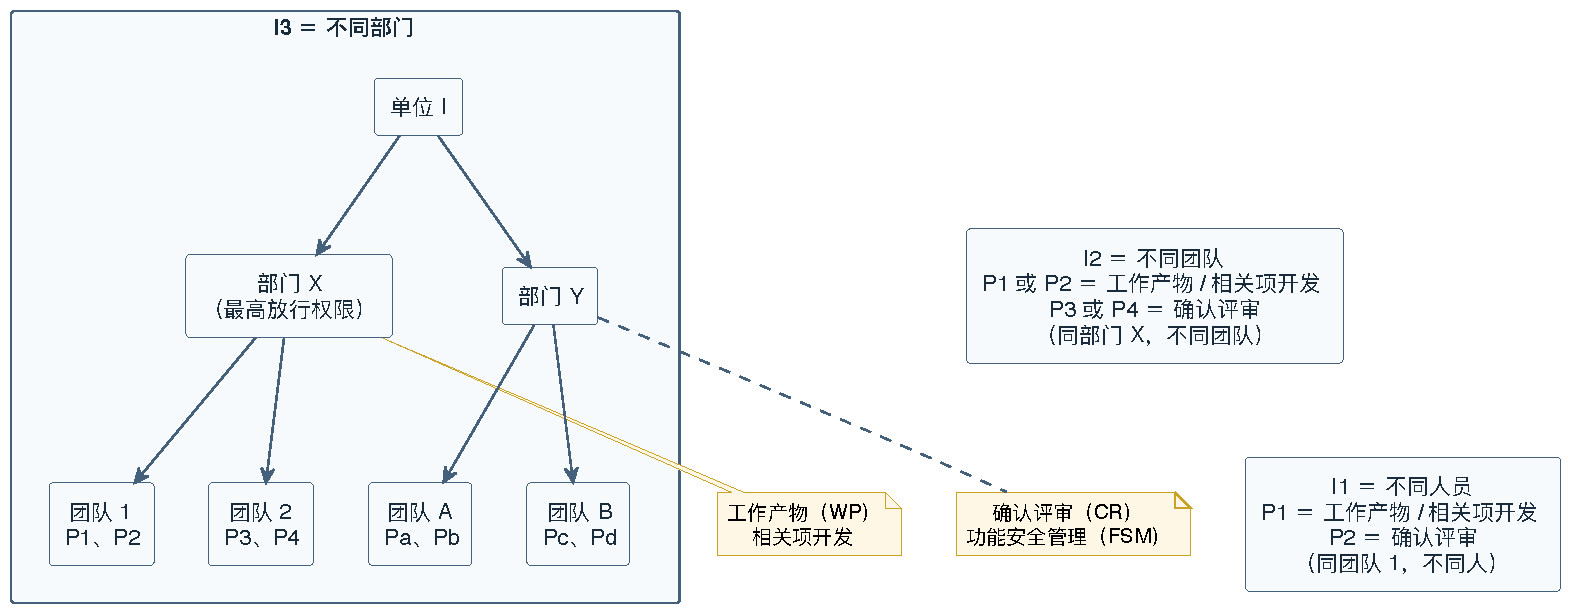
\includegraphics{figures-rendered/appB-fig2-p12-figure3-independence-levels.pdf}}
\setcounter{figure}{1}
\caption{确认评审独立性等级（重绘自 Part 12 Figure 3）——I1 不同人员、I2 不同团队、I3 不同部门：工作产物创建方与确认评审方在组织树上的距离即独立性等级，最高放行权限所在部门做开发、另一部门做评审即 I3。}
\end{figure}

\Needspace{6\baselineskip}
\section{摩托车 HARA 与 MSIL 判定}

\Needspace{5\baselineskip}
\subsection{骨架不变：还是第 4 章那条流水线}

Clause 8 是 Part 12 的技术核心，对应 Part 3 Clause 6。先说继续适用的主要步骤，免得读者以为要重学一遍 HARA：HARA 基于相关项定义（8.4.1.1）；\textbf{评估时不考虑相关项内部的安全机制}——已实现或将实现的安全机制属于功能安全概念，不进 HARA（8.4.1.2，p20）；运行场景与运行模式要覆盖正确使用与可合理预见的误用（8.4.2.1）；危害用 FMEA/HAZOP 等方法系统性识别、在\textbf{整车层面}定义（8.4.2.2/8.4.2.3）；后果要合并评估多功能同时丧失的情形——供电失效可能同时丢“发动机扭矩”与“前照明”（8.4.2.6 EXAMPLE，p21）；运行场景切分过细会不当压低完整性等级，要聚合相似场景（8.4.2.7，p21）；分类有疑义时保守取高（8.4.3.1 NOTE，p21）。这些共通步骤之后，仍须按 Part 12 核对摩托车专用的分类语境、MSIL 输出和映射要求。

预期功能之外的危害同样出界：仅由相关项行为（无失效）引发的危害不在范围内——正常摩托车不被期望高速穿越无铺装路面、不被期望参加公路赛或越野赛（8.4.2.1 NOTE 2 与 EXAMPLE，p21）；超出 ISO 26262 范围的危害按组织自有程序处理（8.4.2.4）。

\Needspace{5\baselineskip}
\subsection{S/E/C：同一副度量衡，换了持秤人}

三个分类参数采用与 Part 3 相同的类目集合：严重度 S0–S3（Table 2，p22）、暴露概率 E0–E4（Table 3，p23）、可控性 C0–C3（Table 4，p24）。共同类目让 MSIL 与 ASIL 的表格关系可以逐项表达；摩托车适配的差异则落在判定语境、证据和后续映射：

\textbf{严重度}：风险评估聚焦每个暴露于风险的人——包括肇事车辆的骑手与乘员，以及骑行者、行人、其他车辆乘员（8.4.3.2 NOTE 1，p22）；伤害刻画可用 \textbf{AIS}（Abbreviated Injury Scale，简明损伤定级）——B.6 展开；\textbf{标准穿戴装备（头盔、护甲、手套、靴子——按用户手册规定）假定在用}（NOTE 5，p22）——这条乘用车没有对应物：四轮的被动安全在车上，两轮的被动安全穿在人身上。三条通用规则保留：多处伤害可合并抬级（NOTE 2）；“差值定级”规则照搬 Part 3——若危害事件只是让本已发生的事故雪上加霜，严重度可取“有失效”与“无失效”两种结局之差（8.4.3.3 的气囊例：不弹出的气囊对应 S3，正常弹出对应 S2，差一级，故该失效可判 S1，p22）；纯财产损失判 S0、免除 MSIL 定级（8.4.3.4）。

\textbf{暴露概率}：装车率不得计入——评估假定每辆车都装了该相关项，“不是每辆车都有这个功能”不构成降 E 的理由（8.4.3.6，p23）；E0 留给“难以置信”的情形（不可抗力如地震、高速路上迫降的飞机），须记录排除理由，判 E0 免除 MSIL 定级（8.4.3.7，p23）。

\textbf{可控性}：这是摩托车 delta 最深的一处。评估对象是骑手\textbf{或其他卷入场景的人}获得足够控制、避免特定伤害的概率（8.4.3.8，p23）；骑手画像有明确假设——状态适宜（不疲劳）、持照且受过训练、了解所骑车辆的操作特性、遵守法规（NOTE 2，p23——对照第 4 章乘用车的“有驾照的普通驾驶员”假设，这里多了“了解车辆特性”一条，因为摩托车之间的动力学差异远大于乘用车之间）；与车辆运动方向/速度无关的危害（如肢体卷入运动部件），可控性改为评估当事人自行脱困或被他人解救的概率（NOTE 3）；涉及多个交通参与者时可综合故障车的可控性与他人的假定动作（NOTE 4）；\textbf{摩托车危害事件的可控性评估方法单列 Annex C}（NOTE 5）——专家骑手与 CCP 在那里登场，B.6 展开；有官方最低性能法规且有实际使用证据支撑时，法规可作为选级理由的一部分（NOTE 6/7，p23）。C0 的用法与乘用车一致：不影响车辆安全运行的功能丧失（部分骑手辅助系统）或常规骑手动作即可避免事故的情形，判 C0 免除 MSIL 定级（8.4.3.9，p24）。

\Needspace{5\baselineskip}
\subsection{MSIL 判定表与映射表：两张表、两种关系}

\textbf{MSIL 判定}（8.4.3.10，Table 5，p24）：按 S\(\times\)E\(\times\)C 查表；当前转录中的 36 个 S1–S3\(\times\)E1–E4\(\times\)C1–C3 单元与 Part 3 Table 4 具有相同索引结构，结果词表则使用 QM/MSIL。最低组合给 QM，S3+E4+C3 顶格给 MSIL D。下表是当前转录；转录所据的两种提取视图同出一份 PDF，关键使用仍应回看原表：

\begingroup\small
\setlength{\tabcolsep}{4pt}
\begin{xltabular}{\linewidth}{@{}XXXXX@{}}
\toprule
严重度 & 暴露 & C1 & C2 & C3 \\
\midrule
\endhead
S1 & E1 & QM & QM & QM \\
S1 & E2 & QM & QM & QM \\
S1 & E3 & QM & QM & A \\
S1 & E4 & QM & A & B \\
S2 & E1 & QM & QM & QM \\
S2 & E2 & QM & QM & A \\
S2 & E3 & QM & A & B \\
S2 & E4 & A & B & C \\
S3 & E1 & QM & QM & A \\
S3 & E2 & QM & A & B \\
S3 & E3 & A & B & C \\
S3 & E4 & B & C & D \\
\bottomrule
\end{xltabular}
\endgroup

单看这张表，你会以为 MSIL 就是 ASIL 换了个字母。真正的 delta 在下一步。\textbf{映射}（8.4.3.11，Table 6，p25）：在定义安全目标\textbf{之前}，MSIL 须映射为 ASIL，以便采用 ISO 26262 其他部的要求——

\begin{center}
\begingroup\small
\setlength{\tabcolsep}{4pt}
\begin{tabularx}{\linewidth}{@{}XX@{}}
\toprule
MSIL & ASIL \\
\midrule
QM & QM \\
A & QM \\
B & A \\
C & B \\
D & C \\
\bottomrule
\end{tabularx}
\endgroup
\end{center}

不要用“整体降一档”代替查表。Table 6 给出的五行事实是：\textbf{QM\(\rightarrow\)QM、MSIL A\(\rightarrow\)QM、MSIL B\(\rightarrow\)ASIL A、MSIL C\(\rightarrow\)ASIL B、MSIL D\(\rightarrow\)ASIL C}。把后四行口头概括成“字母向下一格”只能算作者帮助记忆的说明，它会漏掉 QM\(\rightarrow\)QM，并容易把两个分级体系误说成同一把标尺。三条 NOTE 是这张小表的全部注释，逐条读：映射出的 QM 不等于没事——对应危害事件仍可能有安全后果，仍可为其制定安全需求，QM 只表示质量流程足以管理该风险（NOTE 1）；映射的目的是让摩托车应用以\textbf{最恰当的严格程度}避免不合理残余风险（NOTE 2）——背后是 §8.2 NOTE 的行业基线论证；映射出的 ASIL 是\textbf{最低要求}（NOTE 3，p24–25）——想按更高等级开发没人拦着。

为什么设置这张对齐表？标准给出的依据要克制地复述。§8.2 正文指出摩托车动态行为与其他车辆差异很大，摩托车危害事件的可控性更强调骑手，因此风险评估方法需要适配；紧随其后的 NOTE 又说明，摩托车行业的开发过程与技术方案不同，全球既有技术水平表明直接使用 ASIL 分类并不合适，于是以 MSIL 作为 HARA 输出，再建立 MSIL–ASIL 对齐以使用其他各部要求并容纳行业能力。标准没有把年行驶里程、季节性、恶劣天气回避或“已吸收高风险所以再用 ASIL 会过度要求”列为这张表的正式因果链；这些可以成为研究假设，不能替标准发言。项目能做的是逐行采用 Table 6 并把映射结果作为最低要求，不能以“本行业不同”为由自创另一张映射表。

\textbf{MSIL 与 ASIL 不是同义词}，教材必须把这句话钉死。它们类目同构、判定表同构，但：MSIL 是摩托车 HARA 的原生输出，ASIL 是全系列其他部的通用语言；两者之间隔着一张\textbf{不可逆}的映射表（从 ASIL 反推 MSIL 是多值的：ASIL QM 可能来自 MSIL QM 或 MSIL A）；确认措施的独立性查 Part 12 Table 1 时用的是映射后的 ASIL。建模时（B.7）也因此不能把 MSIL 写成 ASIL 的别名。

\begin{figure}[htbp]
\centering
\adjustbox{max size={\linewidth}{0.78\textheight}}{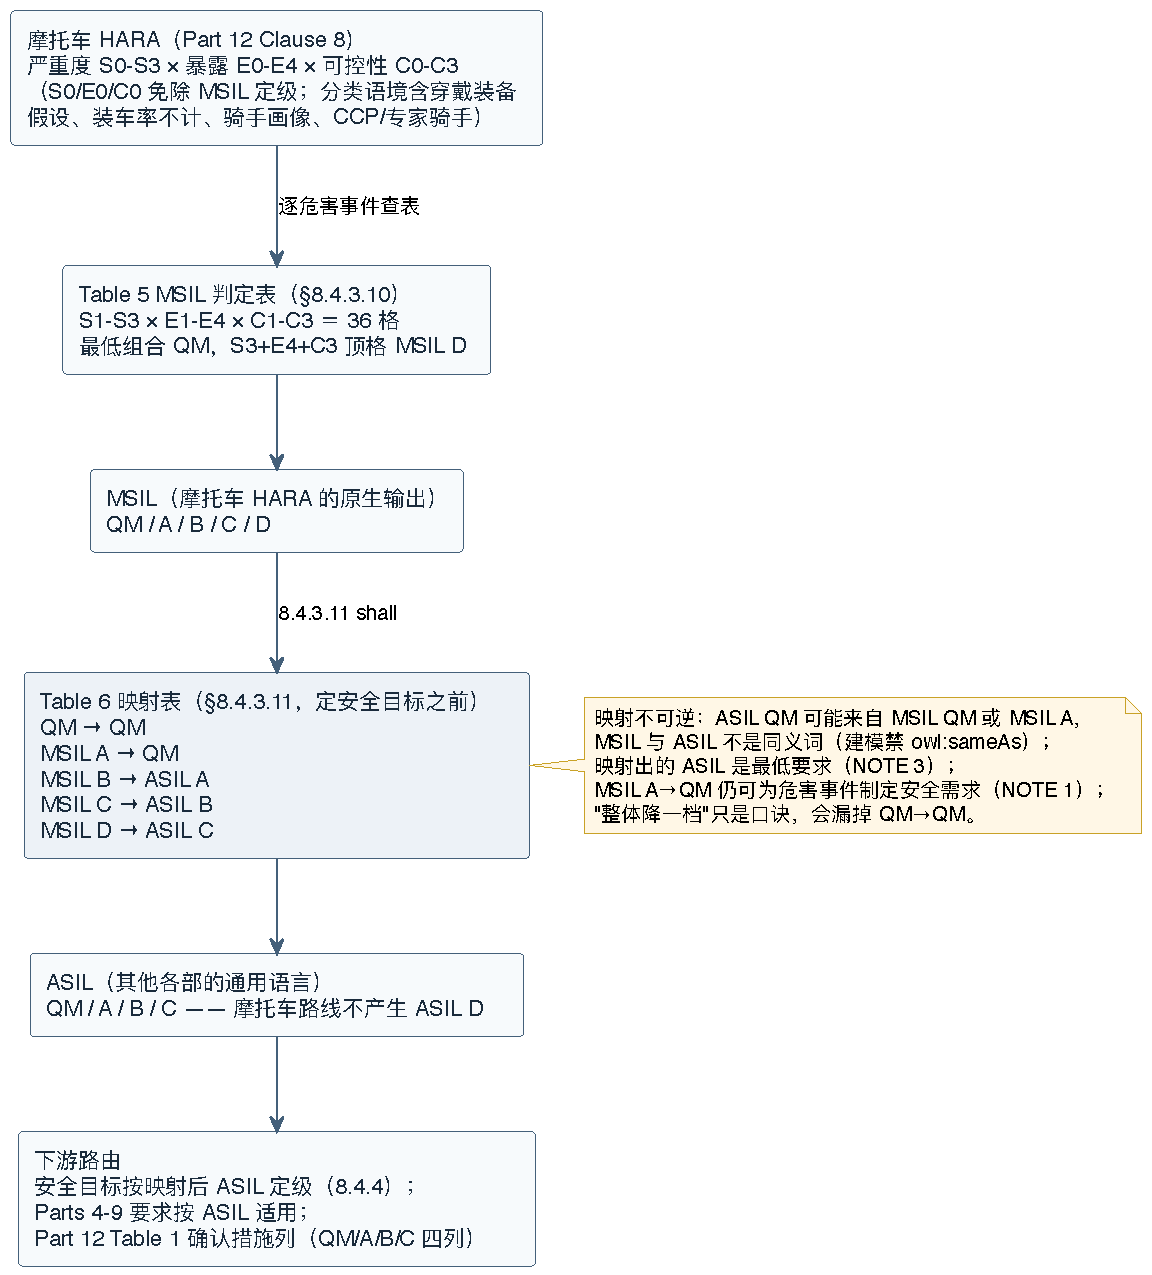
\includegraphics{figures-rendered/appB-fig3-msil-asil-mapping.pdf}}
\setcounter{figure}{2}
\caption{MSIL\(\rightarrow\)ASIL 两表两种关系——S\(\times\)E\(\times\)C 经 Table 5 三十六格判定 MSIL，定安全目标之前经 Table 6 五行（QM\(\rightarrow\)QM、A\(\rightarrow\)QM、B\(\rightarrow\)A、C\(\rightarrow\)B、D\(\rightarrow\)C）映射为 ASIL 再路由下游；映射不可逆、结果为最低要求，摩托车路线不产生 ASIL D。}
\end{figure}

\Needspace{5\baselineskip}
\subsection{安全目标与验证：出口对齐第 4 章}

安全目标的确定沿用第 4 章的主要结构，但增加了摩托车映射与确认语境（8.4.4，p25）：每个带 ASIL（从 MSIL 映射）的危害事件确定一个安全目标，相似安全目标可合并、取最高 ASIL；安全目标按 Part 8 Clause 6 规格化，可含容错时间间隔或物理特征（如非预期加速度上限）；HARA 中使用或产生的假设（骑手动作、外部措施）要识别并\textbf{在 Clause 10 的安全确认中对集成后的相关项验证}（8.4.4.4，p25）。验证要求（8.4.5.1，p25）列了六项证据，前五项与 Part 3 对应，第六项是摩托车特有的 \textbf{MSIL–ASIL 映射一致性}。工作产物为 HARA 报告与其验证报告（8.5，p26）。

\textbf{教学走查}（教学示例，非任何真实项目结论）：摩托车牵引力控制系统，危害事件“正常过弯时非预期扭矩削减”。为演示查表，先显式冻结三项合成输入：E4 的依据只采用 Annex B 明列的“normal cornering”或“slight lean angle or less”；S2 假设来自指定车速、碰撞对象与 AIS 伤情谱分析；C2 假设来自按 CCP 程序形成的代表性骑手可控概率证据。后两项在本附录没有真实事故数据库、速度包络或 CCP 记录，因此只是待证输入，不能说由 Annex B 自动推出。在\textbf{给定这组教学输入}的前提下，查 Table 5 得 \textbf{MSIL B}，再查 Table 6 得 \textbf{ASIL A}，随后可按 ASIL A 查 Parts 4–9 的适用要求和 Part 12 Table 1 的确认措施列。这个算例演示的是特定输入下的查表、映射和后续路由步骤，不确认教学输入在真实项目中成立。

\Needspace{6\baselineskip}
\section{整车集成、测试与安全确认}

\Needspace{5\baselineskip}
\subsection{整车集成与测试：四个测试目标，两条摩托车脚注}

Clause 9 裁剪 Part 4 §7.4.4（§9.1，p26），只动整车集成这一层——第 5 章讲过的集成三层（软硬件、系统、整车）中，前两层照旧走 Part 4。要求主干：相关项集成入整车并执行整车集成测试（9.2.1.1）；相关项与车内通信网络、供电网络的接口规格要验证（9.2.1.2，p26）；测试目标由四张方法表承载（9.2.2，p26–28），列头都是 ASIL A/B/C——又一次，没有 D 列：

\begin{itemize}
\item \textbf{Table 7 功能安全需求的正确实现}（p27）：基于需求的测试、故障注入测试、长期测试、真实条件用户测试，四法对 A/B/C 全部 \nolinkurl{++}；
\item \textbf{Table 8 安全机制的功能表现、准确性与时序}（9.2.2.3，适用于 ASIL (A)(B) 和 C——括号即“对 A、B 是建议”）：性能测试、长期测试、用户测试 \nolinkurl{+/+/++}，故障注入、错误猜测、现场经验派生测试 \nolinkurl{o/+/++}（p27）；
\item \textbf{Table 9 内外接口实现的一致与正确}（9.2.2.4）：内部接口、外部接口、交互/通信测试，均 \nolinkurl{+/+/++}（p28）；
\item \textbf{Table 10 整车级稳健性}（9.2.2.5）：资源占用测试、应力测试、环境条件抗扰与稳健性测试（含 EMC/ESD）、长期测试，均 \nolinkurl{+/+/++}（p28）。
\end{itemize}

四张表的脚注还顺带给了方法定义，几条值得抄进测试计划模板（p27–28）：\textbf{基于需求的测试}针对功能与非功能需求；\textbf{故障注入测试}经专用测试接口或特制元件把故障引入相关项；\textbf{长期测试与真实条件用户测试}类似现场经验测试，但样本更大、由普通用户执行、不受预定测试场景约束；\textbf{错误猜测测试}用专家经验与既往教训定向设计测试；\textbf{性能测试}验证整车层面的容错时间间隔与故障存在时的车辆可控性。摩托车味道正在脚注里：长期测试或用户测试可能不可行；9.2.2.1 NOTE 3 也说明存在骑手安全顾虑时，可以改选测试方法或把活动移到其他子阶段。这里不能把 §4.3 缩成“说明原方法不可行即可”：替换连续条目的方法时，理由必须说明替代方法为何满足对应 requirement；选取备选条目组合时，也必须说明组合或单一方法为何满足对应 requirement。骑手风险解释了为什么换，合规理由还必须解释换完后为什么仍够。

\Needspace{5\baselineskip}
\subsection{安全确认：把 HARA 的假设押回整车上验}

Clause 10 裁剪 Part 4 Clause 8（§10.1，p28）。目标两条：证明安全目标在相关项集成进车辆后达成；证明功能安全概念与技术安全概念对该相关项是恰当的。与验证的分工（§10.2，p29）沿用第 5 章讲过的口径：验证证明“结果符合规格”，确认证明“适合预期用途”——面向一类或一组代表性车辆确认安全措施的充分性。

确认环境（10.4.1，p29）：安全目标在\textbf{整车层面的代表性语境}中确认；代表性车辆按车型与配置选取，HARA 报告可作为选取依据；还要考虑影响技术特征的使用变化。确认规格（10.4.2，p29–30）三要素：\textcircled{\scriptsize 1}受确认的相关项配置（含标定数据，按 Part 6 Annex C；全配置确认不可行时选合理子集）；\textcircled{\scriptsize 2}\textbf{确认程序、测试用例、骑行机动动作与接受准则}；\textcircled{\scriptsize 3}设备与环境条件——“骑行机动动作”（riding manoeuvres）写进规格是摩托车特色：确认场景以机动动作为单位定义。执行（10.4.3，p30）要评估四件事：\textbf{可控性}（用含预期使用与可预见误用的运行场景确认；接受准则可以是“安全状态下的可控性充分”，且单一准则未必够，NOTE 1–3）、外部措施的有效性、其他技术要素的有效性、以及 \textbf{HARA 中影响 ASIL（从 MSIL 映射）的假设}——8.4.4.4 埋的那条线在此收口：机械部件被假定能缓解某 E/E 失效的，其有效性要在整车层面验证（EXAMPLE，p30）。

方法集（10.4.3.4，p30–31）：可重复测试（正向测试、黑盒测试、仿真、边界条件测试、故障注入、耐久、应力、高加速寿命试验 HALT、外部影响仿真）、分析（FMEA/FTA/ETA/仿真）、长期测试（车辆行驶计划、捕获车队——\textbf{对目标用户的长期测试可能不可行}）、真实条件用户测试/盲测/专家小组（\textbf{用户测试可能不可行，真实条件可用仿真条件替代}，NOTE 2，p31）、评审。评价（10.4.4，p31）：确认结果要给出“实现的安全目标为相关项达成功能安全”的证据。工作产物：确认规格（含环境描述）与确认报告（10.5）。

一句对仗收束 B.5：\textbf{测试核对车是否按规格造对，确认评价规格和集成结果是否适合骑手的预期使用}。

\Needspace{6\baselineskip}
\section{附录判例：严重度、暴露度与可控性怎么给证据}

Part 12 的三个资料性附录是判定证据的“教具库”。\textbf{用法纪律先立}：Annex B 开门就声明其示例 for information only 且不穷尽（B.1，p38）；示例代表既往事故分析的期望值，\textbf{不能从个别描述导出普遍结论}（B.2.1，p39）。判例的价值在“证据如何支撑分类”的示范，不在数字本身。

\textbf{风险的解剖}（B.1，p38）：R = F(f, C, S)——风险是危害事件频度、可控性与严重度的函数；频度 f 又拆成“处于可能发生该事件的场景中的概率”（即 E）与“相关项故障率”，后者\textbf{不进 HARA}——完整性等级恰恰是用来事后约束故障率的，这与第 4 章的乘用车逻辑完全一致。

\textbf{严重度判例}（B.2，p39–40）：AIS 把单一伤害分成七级——AIS 0 无伤到 AIS 6 极危重/致命（p39 逐级列出：AIS 1 皮外伤/肌肉痛，AIS 2 深部伤/短暂昏迷/单纯骨折，AIS 3 重伤不危及生命，AIS 4 危及生命但可能存活，AIS 5 存活不确定，AIS 6 极危重如高位颈椎伤及脊髓）；也可换用 MAIS、ISS、NISS 等量表，取决于当时的医学研究水平。Table B.1（p40）把 S 类目翻译成\textbf{概率化的伤情谱}：S0 = AIS 0 且 AIS 1–6 概率小于 10\%（或纯财产损失）；S1 = AIS 1–6 概率大于 10\%（且不到 S2/S3）；S2 = AIS 3–6 概率大于 10\%（且不到 S3）；S3 = AIS 5–6 概率大于 10\%。配套的情景例：步行速度撞路侧设施属 S0 档；市区车速撞路侧设施、步行速度撞行人属 S1 档；主干道车速撞路侧设施、市区车速撞行人、无二次撞击的高速低侧滑属 S2 档；高速公路车速的碰撞、主干道车速被侧面撞击属 S3 档。读法示范：给某危害事件判 S2，理由不该写“感觉挺严重”，而应写“该场景的典型后果谱系对应‘主干道车速与固定物碰撞’，参照事故数据库该类事故 AIS 3–6 概率超过 10\%”。

\textbf{暴露判例}（B.3，p40–43）：E 的两种估法——按\textbf{持续时间}（该场景时长占总运行时间比例：E2 < 1\%，E3 为 1\%–10\%，E4 > 10\%，Table B.2，p42）或按\textbf{频度}（E1 大多数骑手一年不到一次，E2 一年几次，E3 平均骑手一月一次以上，E4 几乎每次骑行，Table B.3，p42–43）。同一场景两种口径可能给出不同档位（如在停车场骑行），取对所分析危害\textbf{更合适}的口径。判例的颗粒度值得学：倾角本身就是分档变量——大倾角 E1、中倾角 E2、小倾角 E3、微倾角 E4；路面条件——冰雪 E1、湿滑树叶/砂石/油污 E2、雨雾湿路 E3；机动动作——故意翘头 E1、紧急制动 E2 档、超车 E3 档、正常过弯 E4 档。还有一条针对“按需动作”设备的公式（p41）：故障可能长期潜伏的（如安全气囊类按需设备），暴露概率按 \(\sigma\) \(\times\) T 估——\(\sigma\) 是场景发生率，T 是故障未被察觉的时长（可长达车辆寿命），该近似在乘积很小时有效；且 HARA 不考虑相关项自带的安全机制来缩短 T（NOTE 2，p41）。

\textbf{可控性判例}（B.4，p43–45）：Table B.4 把 C1/C2/C3 钉在两个分位点上——\textbf{C1：严格多于 99\%} 的代表性骑手或其他交通参与者能避免伤害；\textbf{C2：90\%–99\%}；\textbf{C3：不足 90\%}（p44）。示例矩阵按“危害 \(\times\) 运行场景（括号内为避害动作）”组织，几行典型：失去牵引力——起步加速时（收油、拉离合）判 C0 档，\textbf{压弯加速时}（收油、反打方向、制动）判 C3；非预期减速（相当于发动机制动）——拥堵市区（骑手拉离合、他车制动）判 C0，过弯中（拉离合）判 C1；非预期最大制动——拥堵市区（他车可制动）判 C1，弯道中（反打方向、重心转移）判 C3；前轮非预期抱死——接近停车线（重心转移）与弯道中（转向、重心转移）都判 C3；失去前照明——夜间无照明乡道（减速停车、开远光）判 C1。对照 B.1 的开场故事：\textbf{同一危害换一个机动动作，可控性可以从 C0 跳到 C3}——这就是“运行场景与危害配对分类”而非“给功能整体打分”的原因。NOTE 2 又把边界收紧一圈：这些示例假定中型公路摩托车，评估时要按所考虑车型与性能复核（p44）。

\textbf{可控性评估技术}（Annex C，p46–49）：核心概念是\textbf{可控性分类小组}（CCP）——一个可按项目裁剪人数与构成的评估小组，专长覆盖摩托车可控性评估（由专家骑手执行）、车辆动力学、E/E 系统、功能安全、骑手行为五个方向（C.2，p46）；多组织可共担 CCP，概念阶段即可由 CCP 评估可控性分类，需有理由支撑。为什么不能照搬汽车的“代表性驾驶员群体实测”？C.3 说得直白（p47）：摩托车动力学对人的依赖远超乘用车——稳定性、轨迹与姿态都靠骑手参与维持，骑手的控制行为也与汽车驾驶员截然不同，所以业界通行做法是\textbf{由专家骑手试乘并判断“代表性骑手能否应对”}——专家骑手有经验与技巧处理相当极端的危害事件，但其安全要有充分的风险控制（C.3/C.5，p47–48）。专家骑手不设资格认证标准，由厂商/测试机构/供应商按内部程序选拔，选拔参考项：多年全场景骑行经验、掌握公司标准化可控性分级、有评估经验、能把测试结果\textbf{折算到代表性骑手}、能用技术语言讨论结果、受过公司骑手培训或持公司专家骑手认定（C.4，p47）。四种评估技术（C.5，p47–48）：代表性骑手群体评估（仅适用于不影响稳定性/轨迹/姿态的低风险事件，如电加热把手）；专家骑手评估（Annex C 将其说明为使用频度较高的方法，建议多名专家骑手交叉）；骑行模拟器（真人骑手 + 物理机电动力学台架）；数学建模与仿真（车辆动力学 + 骑手/控制器模型全软件）。Annex C 还说明，对专家骑手也不能以可接受安全水平执行的机动，应分类为 C3（C.5，p48）。评估维度三张小表（C.6，Table C.1–C.3，p48–49）：车辆响应与性能变化（无/轻微/中等/重大）、骑手感知与警觉（不可察觉/可察觉不惊扰/可察觉且惊扰/强烈惊扰，及骑手动作时机从无关紧要到性命攸关）、控制行为（无需改变/正常补偿动作足够/需超出正常补偿/需非凡技巧或超常控制力）——给 C 分级写理由时，可从这三个维度组织证据；具体分级仍要按项目对象、场景和评估记录确认。

\Needspace{6\baselineskip}
\section{本体化实践：MSIL 表的 Semantica 候选合同与未完成边界}

本节把 Part 12 的两张分级表接到第 4 章的判定表模式上，但**不复用 Part 3 专属的
\nolinkurl{iso262:ASILMapping} 契约**。旧本体仓库曾有一套表模型、来源锚、Shape、查询和反例；
它们不在现行书稿中，也没有登记为当前 Semantica built-in package。所以下文只保存
候选 conceptualization 和验收分母，不能描述为“已经落库”或“机器门禁已通过”。

\textbf{先分开分类值与关系类型。} Table 5 继续使用既有的 \nolinkurl{iso262:Severity}、\nolinkurl{iso262:Exposure} 与 \nolinkurl{iso262:Controllability} 受控值，但输出另建为 \nolinkurl{iso262:MSIL_A} 至 \nolinkurl{iso262:MSIL_D}；\nolinkurl{iso262:QM} 可作为两张表的输入或输出，却既不是 MSIL，也不是 ASIL。\nolinkurl{iso262:MSIL} 与 \nolinkurl{iso262:ASIL}、\nolinkurl{iso262:QMClassification} 保持类型不相交。两张表也各有自己的关系类：Table 5 的单元属于 \nolinkurl{iso262:MSILDeterminationMapping}，Table 6 的行属于 \nolinkurl{iso262:MSILToASILMapping}。因此不得把任一单元写成 \nolinkurl{iso262:ASILMapping}，也不得用 \nolinkurl{owl:sameAs} 把 MSIL 与 ASIL 合并。

\textbf{若进入 Semantica，应把两张表登记成两种关系。} 候选
\nolinkurl{iso262:MSILTableRegistry_2018} 分别指向 Table 5 与 Table 6。验收分母必须明确：
Table 5 是 S1–S3 \(\times\) E1–E4 \(\times\) C1–C3 的 \textbf{36 格}；Table 6 是 \textbf{5 行}：QM\(\rightarrow\)QM、
MSIL A\(\rightarrow\)QM、MSIL B\(\rightarrow\)ASIL A、MSIL C\(\rightarrow\)ASIL B、MSIL D\(\rightarrow\)ASIL C。以下 Turtle 只是
\Needspace{8\baselineskip}
书面建模蓝图，不是当前 registry 中可加载的资产：

\nopagebreak[4]
\begin{codebox}
\begin{Verbatim}[fontsize=\small,breaklines=true,breakanywhere=true,breaksymbolleft={},breaksymbolright={}]
iso262:MSIL_T5_S2_E4_C2 a iso262:MSILDeterminationMapping ;
    iso262:inMSILDeterminationTable iso262:MSILDeterminationTable_12_5 ;
    iso262:msilMappingSeverity iso262:S2 ;
    iso262:msilMappingExposure iso262:E4 ;
    iso262:msilMappingControllability iso262:C2 ;
    iso262:msilDeterminationResult iso262:MSIL_B ;
    iso262:hasSourceAnchor iso262:Table_12_5 .

iso262:MSIL_T6_B_A a iso262:MSILToASILMapping ;
    iso262:inMSILToASILTable iso262:MSILToASILTable_12_6 ;
    iso262:mappingMSILSource iso262:MSIL_B ;
    iso262:mappingASILResult iso262:ASIL_A ;
    iso262:hasSourceAnchor iso262:Table_12_6 .
\end{Verbatim}
\end{codebox}

正式迁入时，每张表还必须绑定用户合法持有来源中的物理页、块号与坐标。当前公开书稿
只陈述人工核对过的来源位置，不声称存在 released 机器来源账。即使未来锚点与表单元
同时通过，也仍不会产生项目合规结论。

\textbf{候选验收必须用查询、全量预期集和单因反例守住转录。} 一个合格的未来
Semantica package 至少要检查唯一 registry、36/5 的精确数量、表归属、来源锚点、
属性单值性、S/E/C 组合唯一性、五行映射和 QM/MSIL/ASIL 类型边界，并拒绝
\allowbreak{}\texttt{MSIL\_\allowbreak{}* \allowbreak{}owl:\allowbreak{}same\allowbreak{}As \allowbreak{}ASIL\_\allowbreak{}*}\allowbreak{}。CQ 仍可分三层：单链
\textbf{S3/E4/C3\(\rightarrow\)MSIL D\(\rightarrow\)ASIL C}、36 行 exact bindings、5 行 exact bindings；反例至少
覆盖缺格、重复格、错误结果、缺锚点、缺行和类型偷换。这些是待注册合同，不是已经
执行的 oracle；紧凑分值计算也只能是本书实现选择，不能冒充 ISO 的通用公式。

这里必须把能力边界钉死：**当前没有 released Part 12 package，也没有摩托车项目危害
事件 ABox、HARA 报告、验证报告或 §8.4.5.1 f) 的执行状态实例。** 因而现阶段连
“给定 S/E/C 时两张机器表返回什么”都不能作为 Semantica 执行结果报告，只能回到
正版标准人工核对；更不能回答某项目映射是否已验证。

其余两块仍保持规划态，不能借 Table 5/6 的完成度代替：

\begin{center}
\begingroup\small
\setlength{\tabcolsep}{4pt}
\begin{tabularx}{\linewidth}{@{}XXX@{}}
\toprule
模块 & 当前状态 & 边界 \\
\midrule
Part 12 Table 5/6 MSIL 表模型 & \allowbreak{}\texttt{planned \allowbreak{}/\allowbreak{} \allowbreak{}blocked}\allowbreak{} & 36+5 验收分母保留在书中；尚无 released Semantica package \\
“基线条款\(\rightarrow\)适配 delta\(\rightarrow\)摩托车域适用性”链 & \nolinkurl{planned} & Clause 4.5–10 目前主要是 \nolinkurl{anchor_only} 来源坐标；其余 provision、CQ 与 SHACL 尚未对象化 \\
跨 Parts 1–9 的 T\&B 专属条款账本 & \nolinkurl{planned} & Part 12 §4.6 只提供标记边界；完整条款盘点、覆盖状态与门禁尚未建立 \\
\bottomrule
\end{tabularx}
\endgroup
\end{center}

这一区分决定了当前能发布什么：可以发布本附录的人工阅读快照；不能发布“两张表的
受控机器转录已就绪”“Part 12 全部适配 delta 已可查询”或“T\&B 适配指南已经完成”。

\Needspace{6\baselineskip}
\section{要点回顾与思考题}

\textbf{要点回顾}：

\begin{enumerate}
\item Part 12 是规范性适配：完整基线（Parts 2–9）+ 五处差分（文化/确认措施/HARA/整车集成/安全确认），替代关系精确到条款。
\item Part 12 Table 1 的列是 QM/A/B/C，没有 D；各确认措施的 I0–I3 要逐行读取。“这与 Table 6 最高映射到 ASIL C 相呼应”是教材解释，不是 Table 1 自述的因果结论。
\item 摩托车 HARA 骨架与第 4 章一致；S/E/C 类目不变，判定语境变：穿戴装备假设、装车率不计、骑手画像、专家骑手评估。
\item Table 6 的五行是 QM\(\rightarrow\)QM、MSIL A\(\rightarrow\)QM、B\(\rightarrow\)ASIL A、C\(\rightarrow\)ASIL B、D\(\rightarrow\)ASIL C；这是摩托车域的逐行映射事实，不是可向其他车辆域泛化的“降级算法”，MSIL 与 ASIL 也不是同义词。
\item 整车测试与确认的方法表没有 D 列，长期/用户测试对摩托车可能不可行；HARA 假设应在安全确认中闭环验证，但本书的表模型并不证明某项目已经完成该闭环。
\item Annex B/C 是判例教具：AIS 概率化伤情谱、双口径暴露估计、90\%/99\% 可控性分位点、CCP 与专家骑手。
\item Table 5 的 36 格与 Table 6 的 5 行是未来 Semantica package 的精确验收分母；当前
   尚未 released，适配 delta 语义链也仍为 \nolinkurl{planned/blocked}。
\item T\&B 在 Part 12 里只有标记约定；跨 Parts 1–9 的 T\&B 条款覆盖账本仍为 \nolinkurl{planned}，建成前不能输出完整指南。
\end{enumerate}

\textbf{思考题}（依学习目标设置）：

\begin{enumerate}
\item 【概念辨析】“MSIL B 的系统按 ASIL A 开发，等于摩托车行业给自己放水。”用 §8.2 NOTE、Table 6 的三条 NOTE 与 B.4.3 的论证结构反驳或限定这句话，并指出哪一步论证只有标准委员会有资格做。
\item 【工程推导】教学场景：摩托车电子悬架的危害事件“高速直线行驶中阻尼突变为最硬”。参照 Annex B 的判例组织方式，为 S、E、C 各写一条带证据类型的判定理由（不必给出最终等级），并说明其中哪一条最需要 CCP 介入。
\item 【工程推导】某确认测试计划把 Table 8 中 \nolinkurl{++} 的故障注入测试替换为台架仿真。按 §4.3 的读表规则与 9.2.2.1 NOTE 3，写出这个替换要补的两段论证。
\item 【合同设计题】把下面的 SPARQL 当作未来 Semantica Part 12 package 的\textbf{候选查询蓝图}，人工推演 S2+E4+C2\(\rightarrow\)MSIL B\(\rightarrow\)ASIL A：Table 5 侧使用 \nolinkurl{inMSILDeterminationTable}、\nolinkurl{msilMappingSeverity}、\nolinkurl{msilMappingExposure}、\nolinkurl{msilMappingControllability}、\nolinkurl{msilDeterminationResult}，Table 6 侧使用 \nolinkurl{inMSILToASILTable}、\nolinkurl{mappingMSILSource}、\nolinkurl{mappingASILResult}，并返回两侧 \nolinkurl{hasSourceAnchor}。说明 package 尚未 released 时为什么不能把人工推演写成查询命中；未来即使 exact oracle 通过，也只证明登记图与冻结预期在已编码字段及联接上相符，转录忠实仍须对照受控来源，且结果不能证明 S/E/C 项目输入成立或 §8.4.5.1 f) 已执行。
\end{enumerate}

\nopagebreak[4]
\begin{codebox}
\begin{Verbatim}[fontsize=\small,breaklines=true,breakanywhere=true,breaksymbolleft={},breaksymbolright={}]
PREFIX iso262: <https://w3id.org/iso26262#>
SELECT ?determination ?msil ?conversion ?asil ?anchor5 ?anchor6 WHERE {
  iso262:MSILTableRegistry_2018
      iso262:hasMSILDeterminationTable ?table5 ;
      iso262:hasMSILToASILTable ?table6 .
  ?determination a iso262:MSILDeterminationMapping ;
      iso262:inMSILDeterminationTable ?table5 ;
      iso262:msilMappingSeverity iso262:S2 ;
      iso262:msilMappingExposure iso262:E4 ;
      iso262:msilMappingControllability iso262:C2 ;
      iso262:msilDeterminationResult ?msil ;
      iso262:hasSourceAnchor ?anchor5 .
  ?conversion a iso262:MSILToASILMapping ;
      iso262:inMSILToASILTable ?table6 ;
      iso262:mappingMSILSource ?msil ;
      iso262:mappingASILResult ?asil ;
      iso262:hasSourceAnchor ?anchor6 .
}
\end{Verbatim}
\end{codebox}

\Needspace{6\baselineskip}
\section{回正文索引}

\begingroup\small
\setlength{\tabcolsep}{4pt}
\begin{xltabular}{\linewidth}{@{}XXX@{}}
\toprule
本附录内容 & 回指章节 & 衔接点 \\
\midrule
\endhead
完整基线 + 五处差分的结构（B.2） & ch01/ch03–ch05 & 生命周期总览；被替代条款的宿主章 \\
安全文化七条义务（B.3.1） & ch03 & 安全文化 18 判据 \\
Part 12 Table 1 取代 Part 2 Table 1（B.3.2） & ch03 & 确认措施 I0–I3 与 55 格矩阵 \\
HARA 骨架、S/E/C、切香肠反模式（B.4.1/B.4.2） & ch04 & HARA 首讲、判定表模式 \\
MSIL 判定表与映射表（B.4.3） & ch04 & ASIL 判定表；分级方案变体 \\
安全目标合并与规格化（B.4.4） & ch04/ch05 & SG 出口；Part 8 Clause 6 需求规格 \\
整车集成测试四表（B.5.1） & ch05 & 集成三层与 Part 4 方法表读法 \\
方法表 \nolinkurl{++/+/o} 与括号 ASIL（B.2/B.5） & ch07 & 方法表语义首讲 \\
安全确认与 HARA 假设闭环（B.5.2） & ch04/ch05 & 8.4.4.4 假设\(\rightarrow\)10.4.3.2 验证 \\
AIS/暴露口径/可控性分位点（B.6） & ch04 & S/E/C 证据化判定 \\
MSIL 两关系表模型、CQ 与门禁（B.7） & ch04/ch08 & 判定表形态；来源、类型边界与反例回归 \\
Part 12 delta 与 T\&B 规划边界（B.7） & ch20 & 两项仍为 \nolinkurl{planned}；待补证据清单的验收归属见发布保证章 \\
\bottomrule
\end{xltabular}
\endgroup


*本附录素材：ISO 26262-12:2018 物理页 p9–52；锚点与表格数值经两种同源提取视图交叉定位，仍以原页复核为准。Part 12 正文为规范性适配条款，Annex A/B/C 为资料性判例。*
